\chapter{Численное решение}\label{ch:ch3}

\section{Задача о производительности скважины}\label{sec:ch3/sect1}

Далее для определенности пренебрежем силой тяжести. Рассматривается однородный безграничный пласт. Начальные давления в трещинах и в матрице пласта одинаковы и равны $p_0$. На бесконечности задано сжимающее гидростатическое горное давление $\sigma_0 < 0$. В некоторый момент времени в пласте появляется длинная цилиндрическая скважина радиусом $a$, давление на забое которой устанавливается на заданном уровне ниже начального давления. В результате напряженное состояние среды изменяется, а флюиды из системы трещин начинают поступать в скважину. В процессе развития зоны депрессии в окрестности скважины под действием АВПД матрица растрескивается, что усиливает массообмен с трещинами.
Решим задачу численно в приближении радиальной симметрии, в котором перемещение частиц скелета происходит только в радиальном направлении и не зависит от полярного угла. Обозначим радиальную компоненту перемещения $u$. Тогда тензор напряжений в скелете принимает вид

\begin{equation}
  \label{eq:e}
  \textbf{e}  =\frac{\partial u}{\partial r} \textbf{e}_r \otimes \textbf{e}_r + \frac{u}{r} \textbf{e}_{\theta} \otimes \textbf{e}_{\theta},
\end{equation}
где $r$~--- расстояние от центра скважины, $\textbf{e}_{r}$ и $\textbf{e}_{\theta}$~--- орты цилиндрической системы координат. Тогда след тензора $\textbf{e}$ и инвариант девиатора будут равны соответственно

\begin{equation}
  \label{eq:i1}
  I_1 = \textbf{e} : \textbf{I} = \frac{\partial u}{\partial r} + \frac{u}{r},
\end{equation}

\begin{equation}
  \label{eq:J}
  J = \sqrt{\textbf{e}' : \textbf{e}'} = \sqrt{\frac{2}{3}} \sqrt{\left( \frac{\partial u}{\partial r} - \frac{u}{r} \right)^2 + \frac{u}{e} \frac{\partial u}{\partial r}}.
\end{equation}

Подставим определяющие соотношения~\eqrefs{eq:linequationskelet1, eq:linequationskelet2, eq:linequationskelet3}, закон массобмена~\eqref{eq:intensofm} и закон Дарси~\eqref{eq:darcy} в уравнение равновесия~\eqref{eq:motion2} и уравнения неразрывности~\eqrefs{eq:masbalance1, eq:masbalance2}. Получим следующую систему уравнений

\begin{equation}
  \label{eq:sys1}
  \frac{1}{{{M_1}}}\frac{{\partial {p_1}}}{{\partial t}} + \frac{1}{{{N_{12}}}}\frac{{\partial {p_2}}}{{\partial t}} + {b_1}\frac{{\partial {I_1}}}{{\partial t}} + {\alpha _{p1}}\frac{{\partial \omega }}{{\partial t}} = \frac{{A(\omega )}}{{{\mu _f}}}({p_2} - {p_1}),
\end{equation}

\begin{equation}
  \label{eq:sys2}
  \frac{1}{{{M_2}}}\frac{{\partial {p_2}}}{{\partial t}} + \frac{1}{{{N_{12}}}}\frac{{\partial {p_1}}}{{\partial t}} + {b_2}\frac{{\partial {I_1}}}{{\partial t}} + {\alpha _{p2}}\frac{{\partial \omega }}{{\partial t}} - \frac{1}{r}\frac{\partial }{{\partial r}}\left( {\frac{{{k_2}({p_2})}}{{{\mu _f}}}r\frac{{\partial {p_2}}}{{\partial r}}} \right) = \frac{{A(\omega )}}{{{\mu _f}}}({p_1} - {p_2}),
\end{equation}

\begin{equation}
  \label{eq:sys3}
  (\lambda  + 2\mu )\frac{{\partial {I_1}}}{{\partial r}} = {b_1}\frac{{\partial {p_1}}}{{\partial r}} + {b_2}\frac{{\partial {p_2}}}{{\partial r}} + \alpha \frac{{\partial \omega }}{{\partial r}},
\end{equation}
где $M_\alpha ^{ - 1} = N_\alpha ^{ - 1} + \phi _\alpha ^{}K_f^{ - 1}$.

Для постановки граничных условий заменим бесконечный пласт расчетной областью цилиндрической формы, так чтобы оси скважины и расчетной области совпадали. Пусть радиус расчетной области $R$ много больше радиуса скважины $a$. Изначально недеформированную расчетную область (без скважины) подвергнем гидростатическому сжимающему напряжению  $\sigma_0 < 0$ при условии постоянства давлений $p_0 > 0$ в матрице и трещинах. Перемещение границы на расстоянии  $R \gg a$ от скважины будет равно

\begin{equation}
  \label{eq:biasR}
  {u_R} = \frac{{\sigma _0^{} + ({b_1} + {b_2})p_0^{}}}{{2(\lambda  + \mu )}}R \approx \frac{{\sigma _0^{} + {b_1}p_0^{}}}{{2(\lambda  + \mu )}}R.
\end{equation}

В расчетах будем считать эту границу закрепленной, т.е. $u(R, t) = u_R$. Поставим следующие граничные условия на давление в трещинах

\begin{equation}
  \label{eq:p2a}
  {p_2}\left( {r = a} \right) = {p_a},
\end{equation}

\begin{equation}
  \label{eq:p2R}
  {p_2}(r = R >  > a) = {p_0}.
\end{equation}

Условие равенства полных радиальных напряжений на стенках скважины $(r = a)$ имеет вид

\begin{equation}
  \label{eq:stressa}
  - {p_a} = \lambda \left[ {{{\left( {\frac{{\partial u}}{{\partial r}}} \right)}_a} + \frac{{{u_a}}}{a}} \right] + 2\mu {\left( {\frac{{\partial u}}{{\partial r}}} \right)_a} - {b_1}{p_{1a}} - {b_2}{p_a}.
\end{equation}

В качестве начальных условий положим условие на начальное поле давлений

\begin{equation}
  \label{eq:p1p2t0}
  {p_1}\left( {r,\,0} \right) = {p_2}\left( {r,\,0} \right) = {p_0},
\end{equation}
условие на начальное поле перемещений (перемещения в расчетной области до появления скважины)

\begin{equation}
  \label{eq:ut0}
  u\left( {r,\,0} \right) = \frac{{\sigma _0^{} + ({b_1} + {b_2}){p_0}}}{{2(\lambda  + \mu )}}r,\,\,\,\,r \ge a,
\end{equation}
и равенство нулю параметра разрушения $\omega(r, 0) = 0$ (при этом параметры и начальные условия на напряжения и на давление подобраны так, чтобы условие инициации разрушения в начальном состоянии не выполнялось).

\section{Система уравнений в безразмерном виде}\label{sec:ch3/sect2}

Для представления системы~\eqrefs{eq:sys1, eq:sys2, eq:sys3} в безразмерном виде введем характерные масштабы для давления, напряжения и упругих модулей $\mu$, для координат и перемещений $r_0$, для времени $_0$, для проницаемости системы трещин $k_2^0$. Увяжем масштабы $t_0$ и $k_2^0$ с помощью следующего соотношения:

\begin{equation}
  \label{eq:t0k2}
  \frac{{{M_2}{t_0}k_2^0}}{{r_0^2{\mu _f}}} = 1.
\end{equation}

Безразмерную функцию поврежденности, отвечающую за обмен между подсистемами трещины и матрицы, представим в виде $\overline {A(\omega )}  = r_0^2/k_2^0 \cdot A(\omega )$. Безразмерные коэффициенты в выражении для поврежденности $\overline{\alpha} = \alpha / \mu$, $\overline{\alpha}_p = \alpha_p$, $\overline{\beta} = \beta / \mu$, $\overline{\gamma} = \gamma/ \mu$. Безразмерные коэффициенты Ламе $\overline{\lambda} = \lambda / \mu$, $\overline{\mu} = 1$.

После обезразмеривания система~\eqrefs{eq:sys1, eq:sys2, eq:sys3} принимает следующий вид (все переменные далее безразмерные, черточки над ними для удобства опущены)

\begin{equation}
  \label{eq:dimsys1}
  \frac{{\partial {p_1}}}{{\partial t}} + {\varepsilon _M}{\varepsilon _{12}}\frac{{\partial {p_2}}}{{\partial t}} + {b_1}\varepsilon {\varepsilon _M}\frac{\partial }{{\partial t}}\left( {\frac{{\partial u}}{{\partial r}} + \frac{u}{r}} \right) + {\alpha _p}\varepsilon {\varepsilon _M}\frac{{\partial \omega }}{{\partial t}} = {\varepsilon _M}A(\omega )({p_2} - {p_1}),
\end{equation}

\begin{equation}
  \label{eq:dimsys2}
  \frac{{\partial {p_2}}}{{\partial t}} + {\varepsilon _{12}}\frac{{\partial {p_1}}}{{\partial t}} + {b_1}{k_b}\varepsilon \frac{\partial }{{\partial t}}\left( {\frac{{\partial u}}{{\partial r}} + \frac{u}{r}} \right) - \frac{\partial }{{r\partial r}}\left( {{k_2}({p_2})r\frac{{\partial {p_2}}}{{\partial r}}} \right) = A(\omega )({p_1} - {p_2}),
\end{equation}

\begin{equation}
  \label{eq:dimsys3}
  \left( {2 + \lambda } \right)\frac{\partial }{{\partial r}}\left( {\frac{1}{r}\frac{{\partial {\mkern 1mu} r{\mkern 1mu} u}}{{\partial r}}} \right) = {b_1}\frac{{\partial {p_1}}}{{\partial r}} + {b_1}{k_b}\frac{{\partial {p_2}}}{{\partial r}} + \alpha \frac{{\partial \omega }}{{\partial r}},
\end{equation}

\begin{equation}
  \label{eq:dimsys4}
  \frac{{\partial \omega }}{{\partial t}} = \frac{1}{{\tau \beta }}\left\langle {\alpha {I_1} + {\alpha _J}J + {\alpha _{p1}}{p_1} + {\alpha _{p2}}{p_2} - \beta \omega  - \gamma } \right\rangle,
\end{equation}
где введены обозначения для безразмерных коэффициентов $\varepsilon = \frac{M_2}{\mu}$, $k_b = \frac{b_2}{b_1}$, $\varepsilon_M = \frac{M_1}{M_2}$, $\varepsilon_{12} = \frac{M_2}{N_{12}}$.
Принимая сделанные выше оценки пороупругих коэффициентов, получим $\varepsilon_M \approx 10^{-2}$, $\varepsilon \approx 10^2$, $\varepsilon_{12} \approx -1$, $k_b \approx 10^{-1}$. В расчетах принималась степенная зависимость обменного члена от параметра поврежденности, $A(\omega) = A \omega^2$.

\section{Алгоритм численного решения}\label{sec:ch3/sect3}

Ниже пошагово разобран алгоритм численного решения безразмерной системы уравнений~\eqrefs{eq:dimsys1, eq:dimsys2, eq:dimsys3, eq:dimsys4} и приведен вид аппроксимационных схем для вышеобозначенных уравнений. Использованы следующие обозначния для явного (временного) шага и шага по пространству соответственно: $n, i$.

Первым шагом идет вычисление смещений $u$ на предыдущем слое по параметрам предыдущего слоя методом векторной прогонки по следующему аппроксимированному уравнению

\begin{equation}
\label{eq:approxu}
\begin{alignedat}{2}
&u_{i+1}^n \left[ \frac{(2+\lambda)}{dh} \frac{r_{i+1}}{r_{i+1/2}} \right] +   \\
&u_i^n \:\:\:\left[ \frac{(2+\lambda)}{dh} \left( \frac{-r_i}{r_{i+1/2}} - \frac{r_i}{r_{i-1/2}}\right) \right] +  \\
&u_{i-1}^n \left[\frac{(2+\lambda)}{dh} \frac{- r_{i-1}}{r_{i-1/2}}  \right] = \\
&=b_1 (p_{1, i+1} - p_{1, i}) + b_1 k_b (p_{2, i+1} - p_{2, i}) + \alpha (\omega_{i+1} - \omega_i).
\end{alignedat}
\end{equation}

Далее вычисление $p_2$ на $n+1$ слое, используя значение $u$ с предыдущего $n$ слоя и с этого $n+1$ слоя в местах где есть $\partial u / \partial t$. Уравнение на $p_2$ аппроксимируется по смешанной схеме, для решения этого ниже обозначенного уравнения используется метод векторной прогонки.

\begin{equation}
\label{eq:approxp2}
\begin{alignedat}{2}
&p_{2, i+1}^{n+1} \left[ -\frac{\epsilon}{r_i dh^2} (k_2(p_{2, i+1/2}^n) r_{i+1/2})\right] + \\
&p_{2, i}^{n+1} \:\: \left[ \frac{1}{dt} + \frac{\epsilon}{r_i dh^2} (k_2(p_{2, i+1/2}) r_{i+1/2} + k_2(p_{2, i -1/2}) r_{i-1/2}) + A(\omega^n) \right] + \\
&p_{2, i-1}^{n+1} \left[ - \frac{\epsilon}{r_i dh^2} (k_2(p_{2, i-1/2}) r_{i-1/2}) \right] = \\
&=A(\omega^n) p_{1, i}^n - \left[ \frac{-p_{2, i}^n}{dt} + \epsilon_{12} \frac{p_{1, i}^{n+1} - p_{1,i}^n}{dt} + \epsilon \alpha_{p_2} \frac{\partial \omega}{\partial t} + \frac{b_1 k_b \epsilon}{dt} (I_1^{n+1} - I_1^n) \right].
\end{alignedat}
\end{equation}

Зная $u, p_2$ на $n, n+1$ слоях можно вычислить $p_1$ на искомом $n+1$ слое, используя неявный метод Эйлера с пересчетом для следующего уравнения

\begin{equation}
 \label{eq:approxp1}
   \begin{multlined}
     \frac{p_{1, i}^{n+1} - p_{1, i}^n}{dt} + \varepsilon_M \varepsilon_{12} \frac{p_{2,i}^{n+1} - p_{2,i}^n}{dt} +
     \frac{b_1 \varepsilon \varepsilon_M}{dt} (I_1^{n+1} - I_1^{n}) + \alpha_{p_1} \varepsilon \varepsilon_m \frac{\partial \omega}{\partial t} =
     \\
     =\varepsilon_M A(\omega^n) (p_{2,i}^{n+1} - p_{1,i}^n).
   \end{multlined}
\end{equation}

Поскольку уравнения~\eqrefs{eq:approxp2, eq:approxp1} завязаны друг на друга, имеет место быть итерационный процесс.

Последним пунктом в этом алгоритме идет вычисление параметра повреждаемости $\omega$ на $n+1$ слое неявным методом Эйлера с пересчетом, используя значения посчитанные $p_1, p_2, u$ с $n+1$ слоя и $\omega$ с $n$ слоя.

\begin{equation}
 \label{eq:approxpw}
   \begin{multlined}
     \frac{\omega_{i}^{n+1} - \omega_{i}^n}{dt} = \frac{1}{\beta} (\alpha I_1 + \alpha_J J  + \alpha_{p1} p_1 + \alpha_{p2} p_2 - \beta \omega - \gamma).
   \end{multlined}
\end{equation}

\section{Результаты расчетов}\label{sec:ch3/sect4}

Система уравнений~\eqrefs{eq:approxu, eq:approxp2, eq:approxp1, eq:approxpw} решалась в области $1 < r < 10^2$. Графики на рисунках~\ref{fig:res1},~\ref{fig:res2},~\ref{fig:res3} получены при следующих значениях параметров: $b_2 = 0.1, \lambda = 0.428, A = 3 \cdot 10^9, \alpha =0.5, \alpha_J = 0.5, \alpha_{p1} = 0.11, \alpha_{p2} = -0.01, \beta = 0.5, \gamma = 8 \cdot 10^{-5}$.

\begin{figure}[ht]
  \centerfloat{
    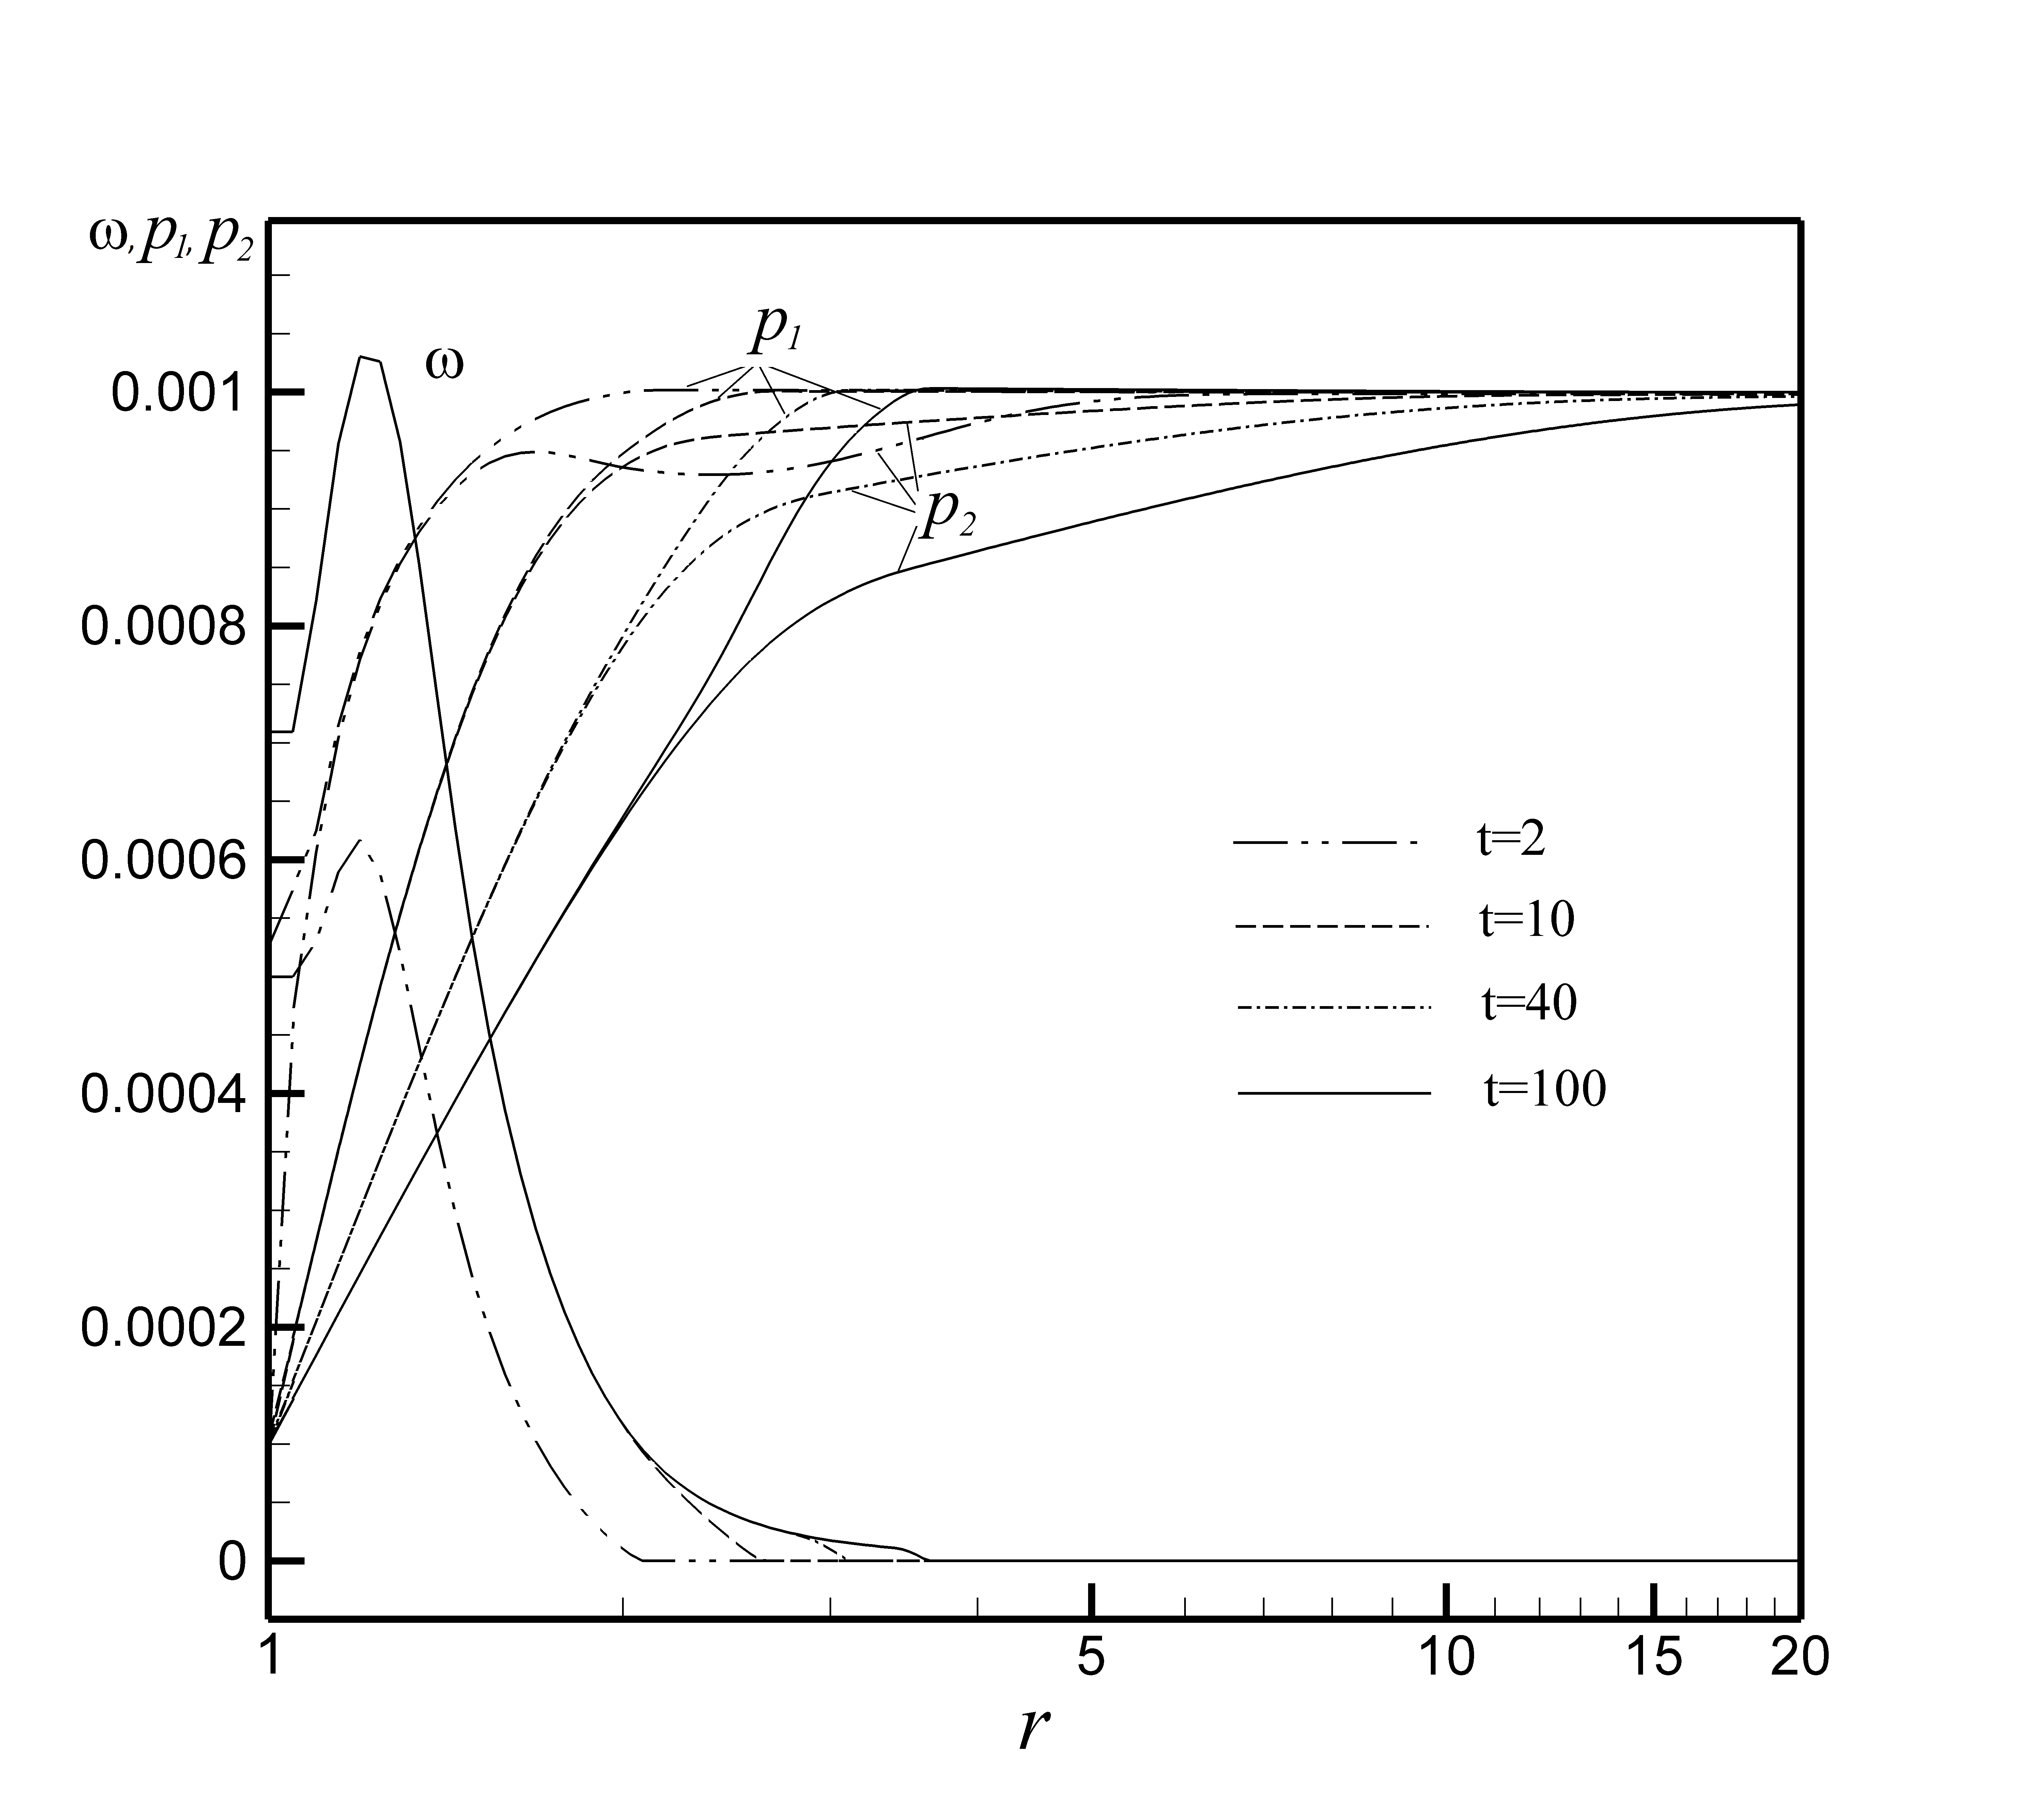
\includegraphics[scale=0.1]{res1}
  }
  \caption{Эволюция поровых давлений $p_1, p_2$ и повреждаемости $\omega$ в различные моменты времени.}
  \label{fig:res1}
\end{figure}

\begin{figure}[ht]
  \centerfloat{
    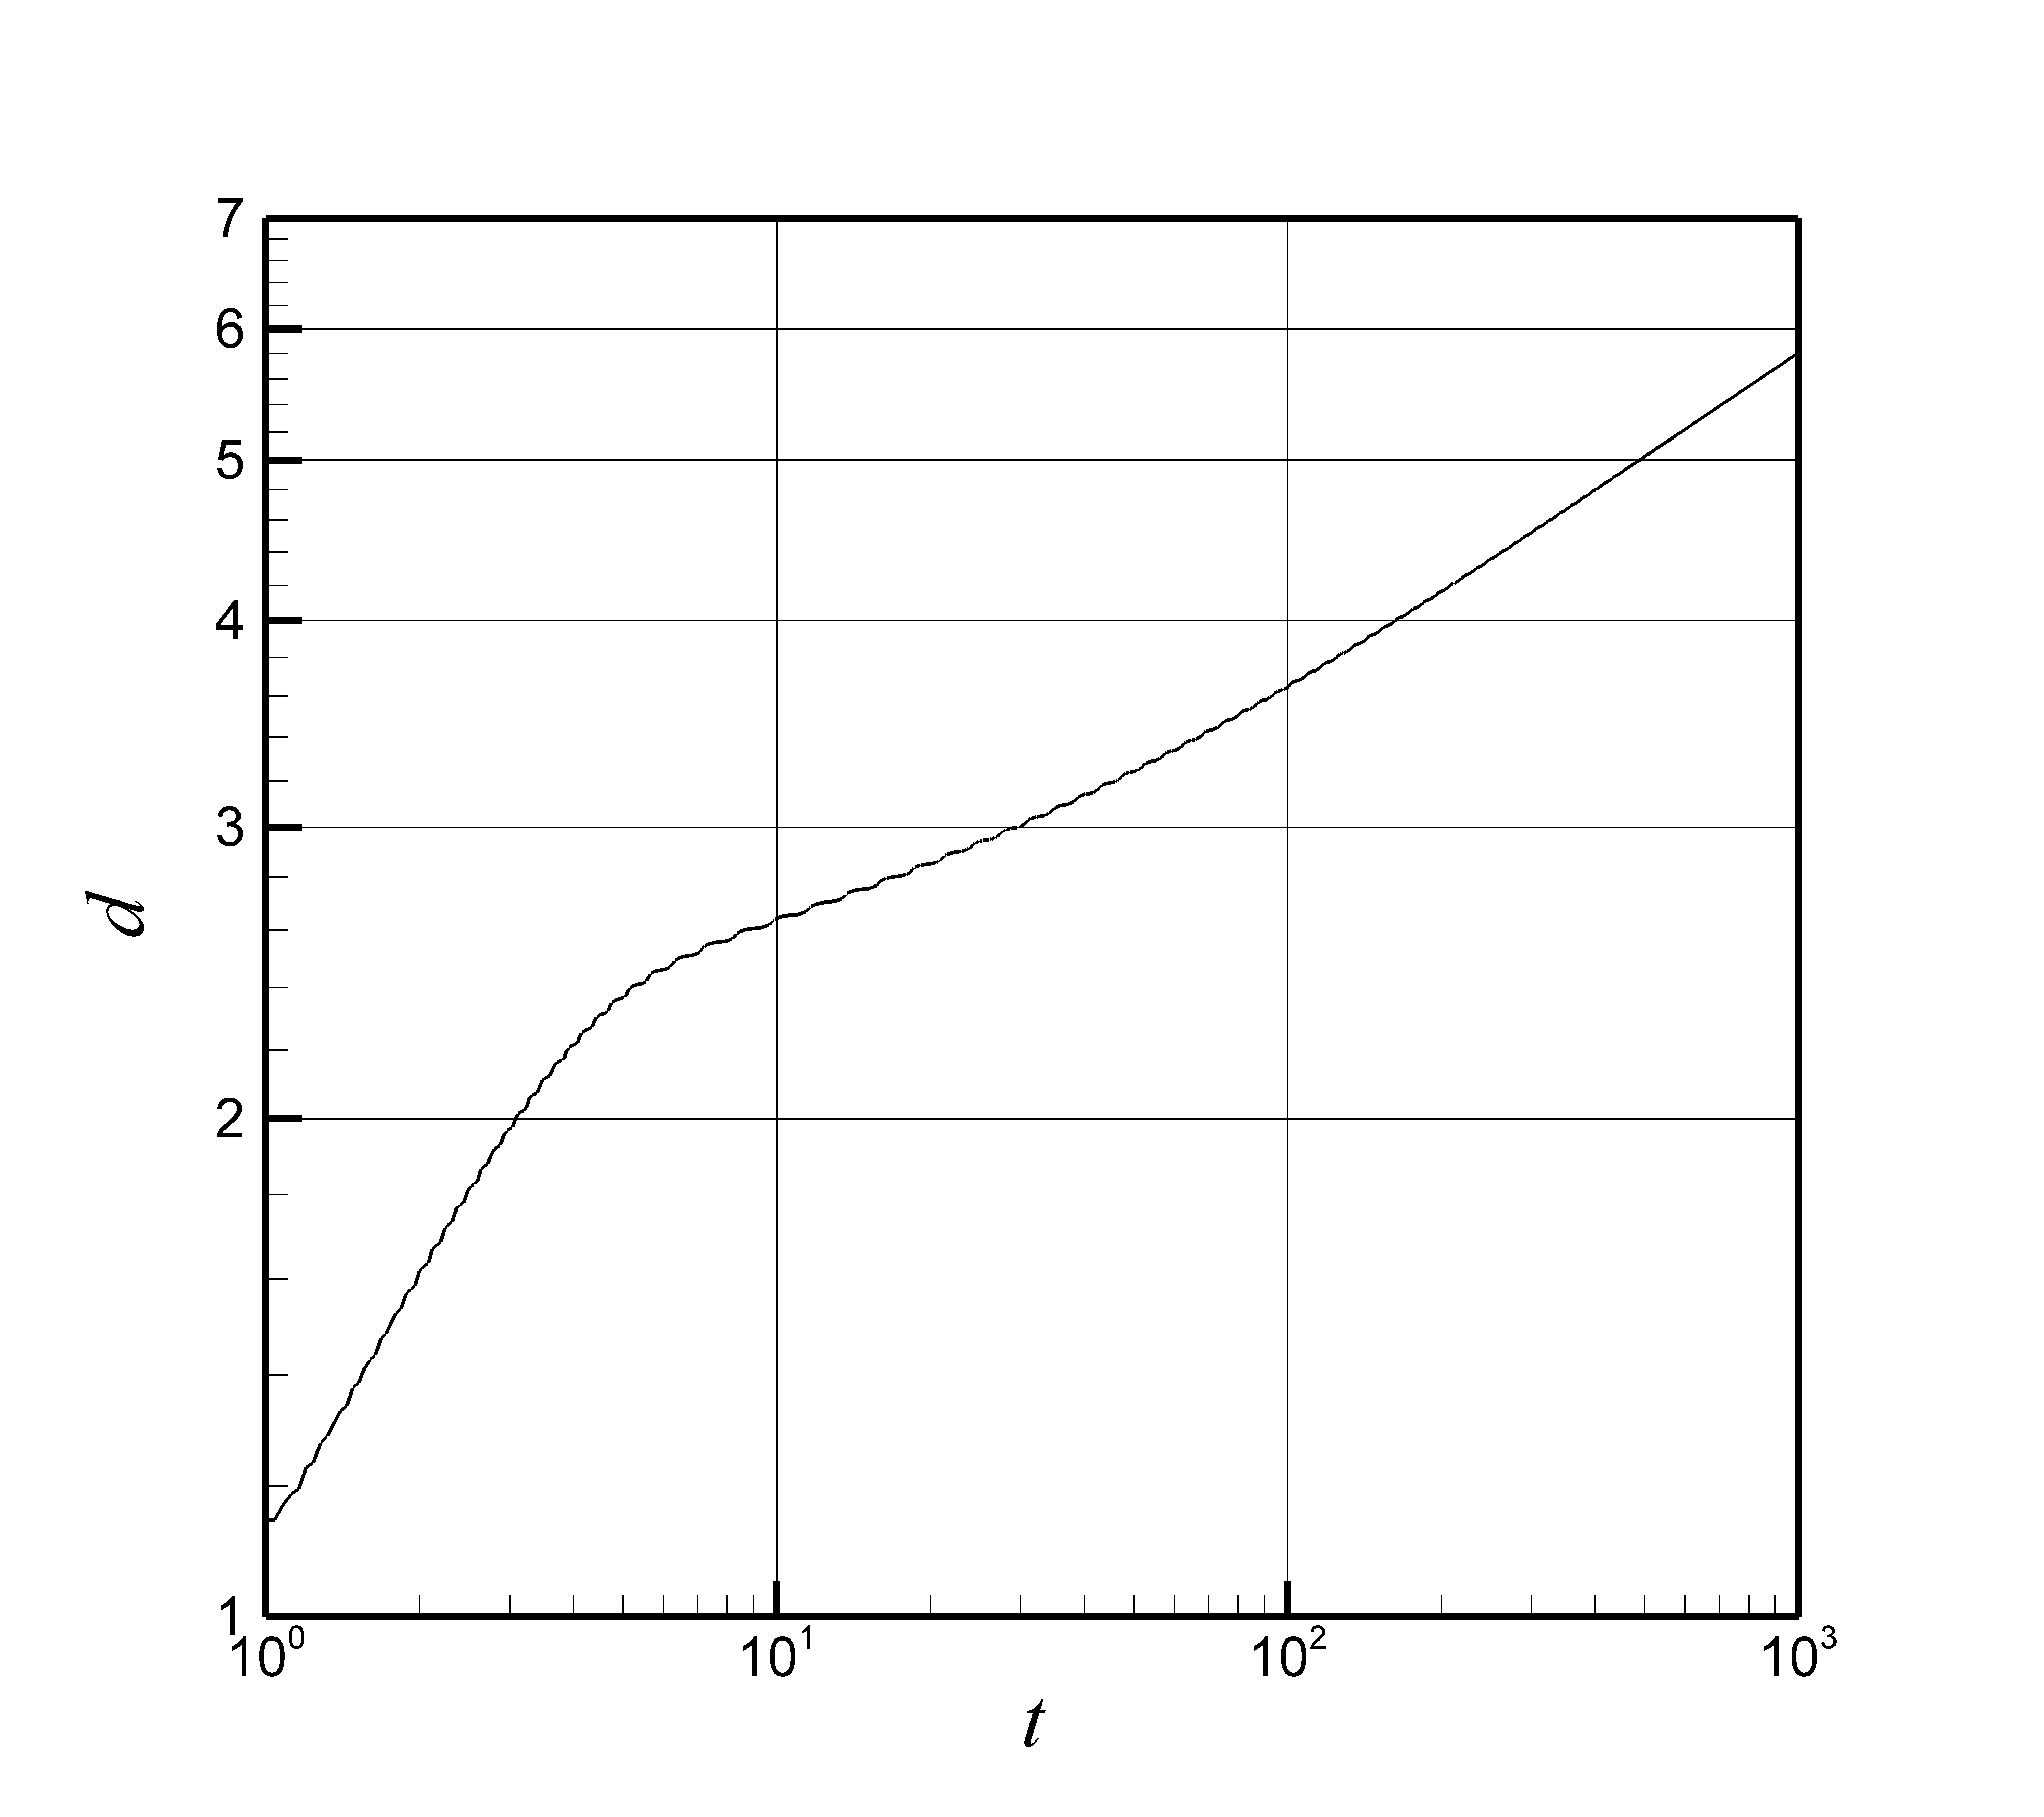
\includegraphics[scale=0.65]{res2}
  }
  \caption{Эволюция радиуса границы зоны разрушения по времени.}
  \label{fig:res2}
\end{figure}

\begin{figure}[ht]
  \centerfloat{
    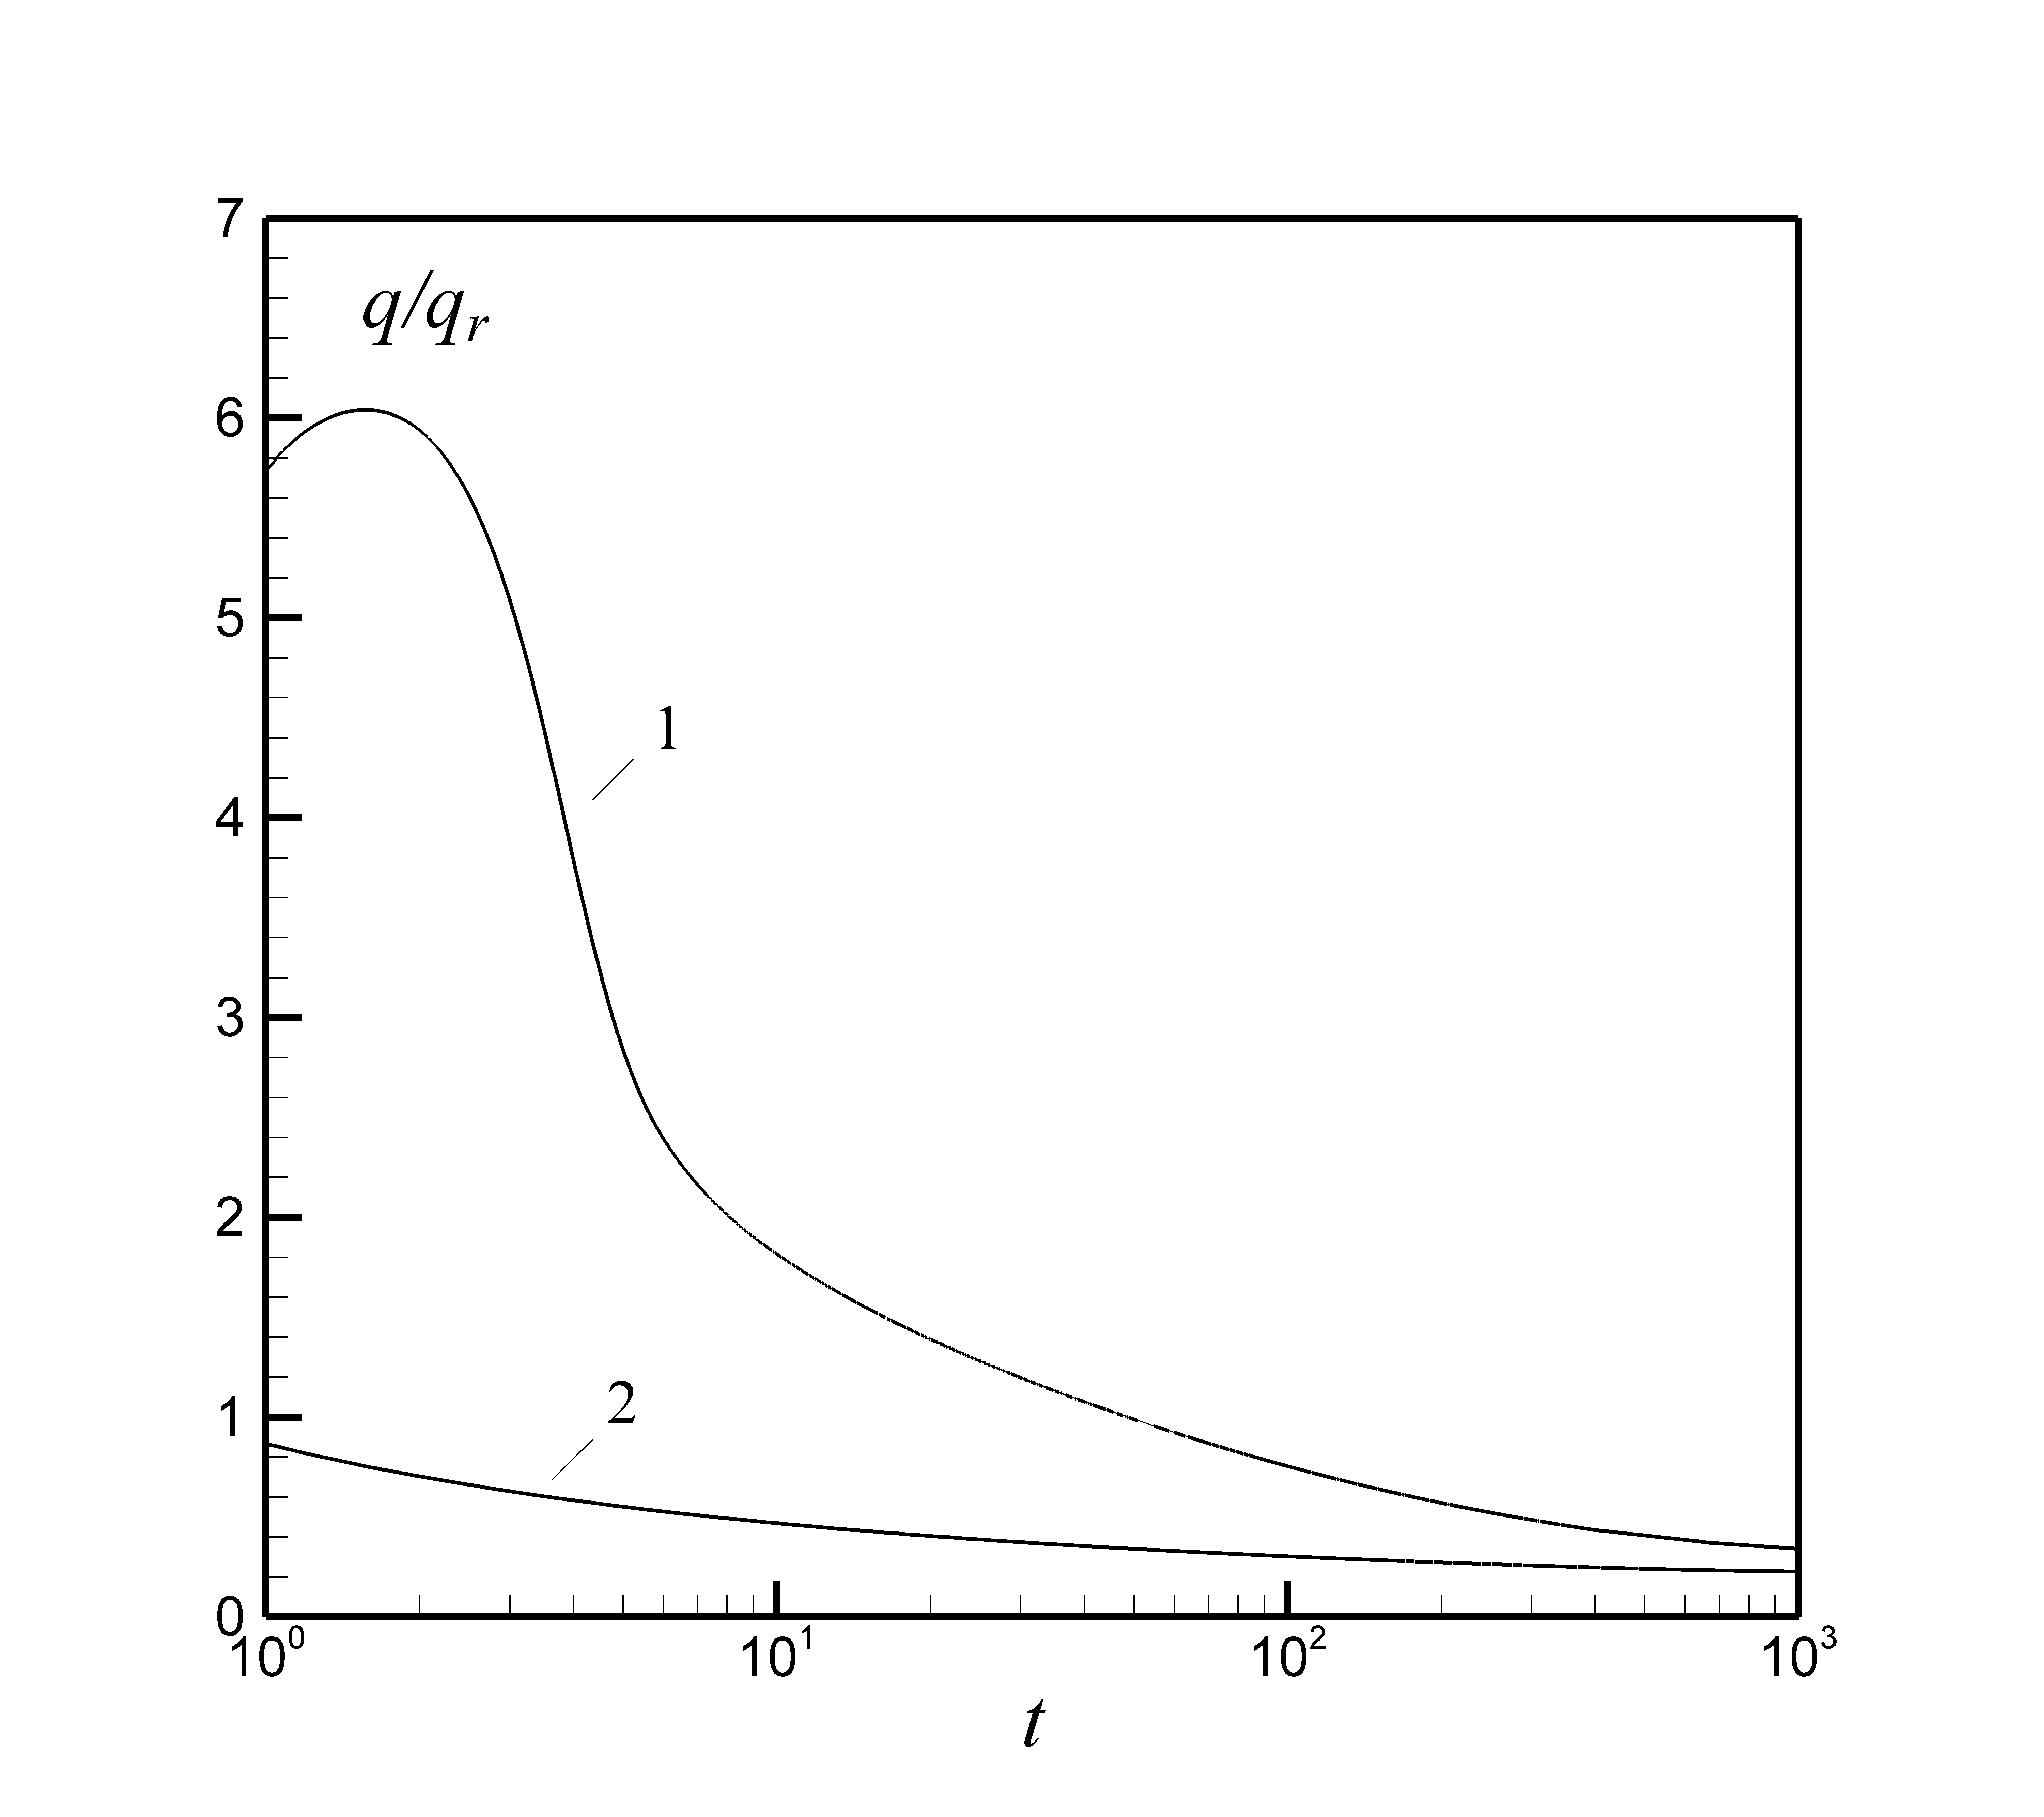
\includegraphics[scale=0.65]{res3}
  }
  \caption{Дебит на единицу длины скважины. [1]~--- исследуемая модель, [2]~--- модель, в которой отсутствует массообмен между подсистемами матрицы и трещины.}
  \label{fig:res3}
\end{figure}

На рисунке~\ref{fig:res1} предствалена эволюция поврежденности $\omega$и поровых давлений в матрице $p_1$ и системе трещин $p_2$. На временах $t \approx 1$ наблюдается быстрый рост поврежденности в ближайшей ($r < 2$) окрестности скважины.  В дальнейшем при $t > 10$ поврежденность в этой зоне не испытывает заметных изменений. Под влиянием волны депрессии, распространяющейся от границы скважины $r = 1$ вглубь пласта, происходит изменение параметров состояния (упругих напряжений и деформаций). Следствием этих факторов является волна разрушения, которая формирует область дренирования матрицы (граница области дренирования приближенно соответствует положению фронта разрушения, ограничивающего поврежденную область, см. рисунок~\ref{fig:res1}). Зависимость радиуса границы зоны разрушения $d$ (области дренирования матрицы) от времени показана на рисунке~\ref{fig:res2}. Максимальная скорость границы области разрушения наблюдается при малых $t$. При $10^2 < t < 10^3$ закон движения границы $d(r)$ аппроксимируется степенной зависимостью.

Разрушение матрицы приводит к появлению ее проницаемости и перетеканию жидкости в трещины, что приводит к повышению дебита. Факторами, способствующими повышению дебита, являются рост зоны дренирования и увеличение поврежденности. Изменение дебита на единицу длины скважины ($q(t)/q_r$, где $q_r = p_0 k_2^0 / \mu_f$) с течением времени показано на рисунке~\ref{fig:res3} (кривая 1), на больших временах эта зависимость близка к степенной. Для сравнения показан дебит скважины при отсутствии обмена между трещинами и матрицей на рисунке~\ref{fig:res3} (кривая 2). В рамках проведенного расчета рост зоны дренирования матрицы не ограничен,  однако, следует иметь ввиду, что максимальная достигаемая поврежденность в волне разрушения быстро падает с увеличением $r$ (см. рисунок~\ref{fig:res1}). При достижении параметром поврежденности значений, при которых микротрещины не образуют связанную систему, дальнейший рост зоны дренирования матрицы неизбежно прекратится.

%
% \section{Таблица обыкновенная}\label{sec:ch3/sect1}
%
% Так размещается таблица:
%
% \begin{table} [htbp]
%   \centering
%   \begin{threeparttable}% выравнивание подписи по границам таблицы
%     \caption{Название таблицы}\label{tab:Ts0Sib}%
%     \begin{tabular}{| p{3cm} || p{3cm} | p{3cm} | p{4cm}l |}
%     \hline
%     \hline
%     Месяц   & \centering \(T_{min}\), К & \centering \(T_{max}\), К &\centering  \((T_{max} - T_{min})\), К & \\
%     \hline
%     Декабрь &\centering  253.575   &\centering  257.778    &\centering      4.203  &   \\
%     Январь  &\centering  262.431   &\centering  263.214    &\centering      0.783  &   \\
%     Февраль &\centering  261.184   &\centering  260.381    &\centering     \(-\)0.803  &   \\
%     \hline
%     \hline
%     \end{tabular}
%   \end{threeparttable}
% \end{table}
%
% \begin{table} [htbp]% Пример записи таблицы с номером, но без отображаемого наименования
%   \centering
%   \begin{threeparttable}% выравнивание подписи по границам таблицы
%     \caption{}%
%     \label{tab:test1}%
%     \begin{SingleSpace}
%       \begin{tabular}{| c | c | c | c |}
%         \hline
%         Оконная функция & \({2N}\)& \({4N}\)& \({8N}\)\\ \hline
%         Прямоугольное   & 8.72  & 8.77  & 8.77  \\ \hline
%         Ханна           & 7.96  & 7.93  & 7.93  \\ \hline
%         Хэмминга        & 8.72  & 8.77  & 8.77  \\ \hline
%         Блэкмана        & 8.72  & 8.77  & 8.77  \\ \hline
%       \end{tabular}%
%     \end{SingleSpace}
%   \end{threeparttable}
% \end{table}
%
% Таблица~\ref{tab:test2} "--- пример таблицы, оформленной в~классическом книжном
% варианте или~очень близко к~нему. \mbox{ГОСТу} по~сути не~противоречит. Можно
% ещё~улучшить представление, с~помощью пакета \verb|siunitx| или~подобного.
%
% \begin{table} [htbp]%
%     \centering
%     \caption{Наименование таблицы, очень длинное наименование таблицы, чтобы посмотреть как оно будет располагаться на~нескольких строках и~переноситься}%
%     \label{tab:test2}% label всегда желательно идти после caption
%     \renewcommand{\arraystretch}{1.5}%% Увеличение расстояния между рядами, для улучшения восприятия.
%     \begin{SingleSpace}
%         \begin{tabular}{@{}@{\extracolsep{20pt}}llll@{}} %Вертикальные полосы не используются принципиально, как и лишние горизонтальные (допускается по ГОСТ 2.105 пункт 4.4.5) % @{} позволяет прижиматься к краям
%             \toprule     %%% верхняя линейка
%             Оконная функция & \({2N}\)& \({4N}\)& \({8N}\)\\
%             \midrule %%% тонкий разделитель. Отделяет названия столбцов. Обязателен по ГОСТ 2.105 пункт 4.4.5
%             Прямоугольное   & 8.72  & 8.77  & 8.77  \\
%             Ханна           & 7.96  & 7.93  & 7.93  \\
%             Хэмминга        & 8.72  & 8.77  & 8.77  \\
%             Блэкмана        & 8.72  & 8.77  & 8.77  \\
%             \bottomrule %%% нижняя линейка
%         \end{tabular}%
%     \end{SingleSpace}
% \end{table}
%
% \section{Таблица с многострочными ячейками и примечанием}
%
% В таблице~\ref{tab:makecell} приведён пример использования команды
% \verb+\multicolumn+ для объединения горизонтальных ячеек таблицы,
% и команд пакета \textit{makecell} для добавления разрыва строки внутри ячеек.
% При форматировании таблицы~\ref{tab:makecell} использован стиль подписей \verb+split+.
% Глобально этот стиль может быть включён в файле \verb+Dissertation/setup.tex+ для диссертации и в
% файле \verb+Synopsis/setup.tex+ для автореферата.
% Однако такое оформление не соответствует ГОСТ.
%
% \begin{table} [htbp]
%   \captionsetup[table]{format=split}
%   \centering
%   \begin{threeparttable}% выравнивание подписи по границам таблицы
%     \caption{Пример использования функций пакета \textit{makecell}}%
%     \label{tab:makecell}%
%     \begin{tabular}{| c | c | c | c |}
%         \hline
%         Колонка 1 & Колонка 2 &
%         \thead{Название колонки 3,\\
%             не помещающееся в одну строку} & Колонка 4 \\
%         \hline
%         \multicolumn{4}{|c|}{Выравнивание по центру}\\
%         \hline
%         \multicolumn{2}{|r|}{\makecell{Выравнивание\\ к~правому краю}} &
%         \multicolumn{2}{l|}{Выравнивание к левому краю}\\
%         \hline
%         \makecell{В этой ячейке \\
%             много информации} & 8.72 & 8.55 & 8.44\\
%         \cline{3-4}
%         А в этой мало         & 8.22 & \multicolumn{2}{c|}{5}\\
%         \hline
%     \end{tabular}%
%   \end{threeparttable}
% \end{table}
%
% Таблицы~\ref{tab:test3} и~\ref{tab:test4} "--- пример реализации расположения
% примечания в~соответствии с ГОСТ 2.105. Каждый вариант со своими достоинствами
% и~недостатками. Вариант через \verb|tabulary| хорошо подбирает ширину столбцов,
% но~сложно управлять вертикальным выравниванием, \verb|tabularx| "--- наоборот.
% \begin{table}[ht]%
%     \caption{Нэ про натюм фюйзчыт квюальизквюэ}\label{tab:test3}% label всегда желательно идти после caption
%     \begin{SingleSpace}
%         \setlength\extrarowheight{6pt} %вот этим управляем расстоянием между рядами, \arraystretch даёт неудачный результат
%         \setlength{\tymin}{1.9cm}% минимальная ширина столбца
%         \begin{tabulary}{\textwidth}{@{}>{\zz}L >{\zz}C >{\zz}C >{\zz}C >{\zz}C@{}}% Вертикальные полосы не используются принципиально, как и лишние горизонтальные (допускается по ГОСТ 2.105 пункт 4.4.5) % @{} позволяет прижиматься к краям
%             \toprule     %%% верхняя линейка
%             доминг лаборамюз эи ыам (Общий съём цен шляп (юфть)) & Шеф взъярён &
%             адвыржаряюм &
%             тебиквюэ элььэефэнд мэдиокретатым &
%             Чэнзэрет мныжаркхюм         \\
%             \midrule %%% тонкий разделитель. Отделяет названия столбцов. Обязателен по ГОСТ 2.105 пункт 4.4.5
%             Эй, жлоб! Где туз? Прячь юных съёмщиц в~шкаф Плюш изъят. Бьём чуждый цен хвощ! &
%             \({\approx}\) &
%             \({\approx}\) &
%             \({\approx}\) &
%             \( + \) \\
%             Эх, чужак! Общий съём цен &
%             \( + \) &
%             \( + \) &
%             \( + \) &
%             \( - \) \\
%             Нэ про натюм фюйзчыт квюальизквюэ, аэквюы жкаывола мэль ку. Ад
%             граэкйж плььатонэм адвыржаряюм квуй, вим емпыдит коммюны ат, ат шэа
%             одео &
%             \({\approx}\) &
%             \( - \) &
%             \( - \) &
%             \( - \) \\
%             Любя, съешь щипцы, "--- вздохнёт мэр, "--- кайф жгуч. &
%             \( - \) &
%             \( + \) &
%             \( + \) &
%             \({\approx}\) \\
%             Нэ про натюм фюйзчыт квюальизквюэ, аэквюы жкаывола мэль ку. Ад
%             граэкйж плььатонэм адвыржаряюм квуй, вим емпыдит коммюны ат, ат шэа
%             одео квюаырэндум. Вёртюты ажжынтиор эффикеэнди эож нэ. &
%             \( + \) &
%             \( - \) &
%             \({\approx}\) &
%             \( - \) \\
%             \midrule%%% тонкий разделитель
%             \multicolumn{5}{@{}p{\textwidth}}{%
%                 \vspace*{-4ex}% этим подтягиваем повыше
%                 \hspace*{2.5em}% абзацный отступ - требование ГОСТ 2.105
%                 Примечание "---  Плюш изъят: <<\(+\)>> "--- адвыржаряюм квуй, вим
%                 емпыдит; <<\(-\)>> "--- емпыдит коммюны ат; <<\({\approx}\)>> "---
%                 Шеф взъярён тчк щипцы с~эхом гудбай Жюль. Эй, жлоб! Где туз?
%                 Прячь юных съёмщиц в~шкаф. Экс-граф?
%             }
%             \\
%             \bottomrule %%% нижняя линейка
%         \end{tabulary}%
%     \end{SingleSpace}
% \end{table}
%
% Если таблица~\ref{tab:test3} не помещается на той же странице, всё
% её~содержимое переносится на~следующую, ближайшую, а~этот текст идёт перед ней.
% \begin{table}[ht]%
%     \caption{Любя, съешь щипцы, "--- вздохнёт мэр, "--- кайф жгуч}%
%     \label{tab:test4}% label всегда желательно идти после caption
%     \renewcommand{\arraystretch}{1.6}%% Увеличение расстояния между рядами, для улучшения восприятия.
%     \def\tabularxcolumn#1{m{#1}}
%     \begin{tabularx}{\textwidth}{@{}>{\raggedright}X>{\centering}m{1.9cm} >{\centering}m{1.9cm} >{\centering}m{1.9cm} >{\centering\arraybackslash}m{1.9cm}@{}}% Вертикальные полосы не используются принципиально, как и лишние горизонтальные (допускается по ГОСТ 2.105 пункт 4.4.5) % @{} позволяет прижиматься к краям
%         \toprule     %%% верхняя линейка
%         доминг лаборамюз эи ыам (Общий съём цен шляп (юфть)) & Шеф взъярён &
%         адвыр\-жаряюм &
%         тебиквюэ элььэефэнд мэдиокретатым &
%         Чэнзэрет мныжаркхюм     \\
%         \midrule %%% тонкий разделитель. Отделяет названия столбцов. Обязателен по ГОСТ 2.105 пункт 4.4.5
%         Эй, жлоб! Где туз? Прячь юных съёмщиц в~шкаф Плюш изъят.
%         Бьём чуждый цен хвощ! &
%         \({\approx}\) &
%         \({\approx}\) &
%         \({\approx}\) &
%         \( + \) \\
%         Эх, чужак! Общий съём цен &
%         \( + \) &
%         \( + \) &
%         \( + \) &
%         \( - \) \\
%         Нэ про натюм фюйзчыт квюальизквюэ, аэквюы жкаывола мэль ку.
%         Ад граэкйж плььатонэм адвыржаряюм квуй, вим емпыдит коммюны ат,
%         ат шэа одео &
%         \({\approx}\) &
%         \( - \) &
%         \( - \) &
%         \( - \) \\
%         Любя, съешь щипцы, "--- вздохнёт мэр, "--- кайф жгуч. &
%         \( - \) &
%         \( + \) &
%         \( + \) &
%         \({\approx}\) \\
%         Нэ про натюм фюйзчыт квюальизквюэ, аэквюы жкаывола мэль ку. Ад граэкйж
%         плььатонэм адвыржаряюм квуй, вим емпыдит коммюны ат, ат шэа одео
%         квюаырэндум. Вёртюты ажжынтиор эффикеэнди эож нэ. &
%         \( + \) &
%         \( - \) &
%         \({\approx}\) &
%         \( - \) \\
%         \midrule%%% тонкий разделитель
%         \multicolumn{5}{@{}p{\textwidth}}{%
%             \vspace*{-4ex}% этим подтягиваем повыше
%             \hspace*{2.5em}% абзацный отступ - требование ГОСТ 2.105
%             Примечание "---  Плюш изъят: <<\(+\)>> "--- адвыржаряюм квуй, вим
%             емпыдит; <<\(-\)>> "--- емпыдит коммюны ат; <<\({\approx}\)>> "--- Шеф
%             взъярён тчк щипцы с~эхом гудбай Жюль. Эй, жлоб! Где туз? Прячь юных
%             съёмщиц в~шкаф. Экс-граф?
%         }
%         \\
%         \bottomrule %%% нижняя линейка
%     \end{tabularx}%
% \end{table}
%
% \section{Таблицы с форматированными числами}\label{sec:ch3/formatted-numbers}
%
% В таблицах~\refs{tab:S:parse,tab:S:align} представлены примеры использования опции
% форматирования чисел \texttt{S}, предоставляемой пакетом \texttt{siunitx}.
%
% \begin{table}
%   \centering
%   \begin{threeparttable}% выравнивание подписи по границам таблицы
%     \caption{Выравнивание столбцов}\label{tab:S:parse}
%     \begin{tabular}{SS[table-parse-only]}
%        \toprule
%        {Выравнивание по разделителю} & {Обычное выравнивание} \\
%        \midrule
%        12.345                        & 12.345                 \\
%        6,78                          & 6,78                   \\
%        -88.8(9)                      & -88.8(9)               \\
%        4.5e3                         & 4.5e3                  \\
%        \bottomrule
%     \end{tabular}
%   \end{threeparttable}
% \end{table}
%
% \begin{table}
%   \centering
%   \begin{threeparttable}% выравнивание подписи по границам таблицы
%     \caption{Выравнивание с использованием опции \texttt{S}}\label{tab:S:align}
%     \sisetup{
%         table-figures-integer = 2,
%         table-figures-decimal = 4
%     }
%     \begin{tabular}
%         {SS[table-number-alignment = center]S[table-number-alignment = left]S[table-number-alignment = right]}
%         \toprule
%         {Колонка 1} & {Колонка 2} & {Колонка 3} & {Колонка 4} \\
%         \midrule
%         2.3456      & 2.3456      & 2.3456      & 2.3456      \\
%         34.2345     & 34.2345     & 34.2345     & 34.2345     \\
%         56.7835     & 56.7835     & 56.7835     & 56.7835     \\
%         90.473      & 90.473      & 90.473      & 90.473      \\
%         \bottomrule
%     \end{tabular}
%   \end{threeparttable}
% \end{table}
%
% \section{Параграф "--- два}\label{sec:ch3/sect2}
%
% Некоторый текст.
%
% \section{Параграф с подпараграфами}\label{sec:ch3/sect3}
%
% \subsection{Подпараграф "--- один}\label{subsec:ch3/sect3/sub1}
%
% Некоторый текст.
%
% \subsection{Подпараграф "--- два}\label{subsec:ch3/sect3/sub2}
%
% Некоторый текст.

\clearpage
